\subsection{\textit{Parameter-Efficient Fine-Tuning of Large-Scale
Pre-Trained Language Models}}

Penelitian yang dilakukan oleh \citeauthor{peft_on_plm} membandingkan secara komprehensif terkait metode \textit{transfer-learning} yang efisien secara parameter pada \textit{pre-trained model}. Metode ini disebut sebagai \textit{delta-tuning} pada penelitan tersebut, dengan kata 'delta' muncul dari notasi matematika yang merepresentasikan perubahan \parencite{peft_on_plm}. Metode \textit{delta-tuning} yang digunakan adalah \textit{prompt-tuning} (PT), \textit{prefix-tuning} (PF), LoRA (LR), dan \textit{adapter} (AP). \textit{Delta-tuning} tersebut akan dibandingkan dengan \textit{fine-tuning} (FT) tradisional.

Eksperimen yang dilakukan pada penelitian tersebut dilakukan pada model T5 dengan konfigurasi BASE dan LARGE. Evaluasi metode \textit{delta-tuning} pada model T5 dilakukan pada 100 tugas pemrosesan bahasa alami yang diambil dari \textit{dataset} Huggingface. Tugas yang dipilih termasuk \textit{text classification}, \textit{question answering}, dan \textit{generation}.

Berdasarkan hasil yang didapatkan pada eksperimen tersebut, metode \textit{delta-tuning} dengan pengurangan jumlah parameter yang dilatih dibandingkan dengan \textit{fine-tuning} memberikan hasil yang hampir setara pada sebagian besar tugas. Metode \textit{prefix-tuning}, LoRA, dan \textit{adapter} secara kinerja hampir mirip antara satu sama lain. Bahkan, metode \textit{delta-tuning} pada sebagian tugas mampu memberikan hasil yang dominan dibanding \textit{fine-tuning}. Secara keseluruhan, kinerja pada setiap metode dapat diurutkan sebagai berikut.

\begin{enumerate}
    \item \textit{Fine-Tuning} (FT)
    \item \textit{Low-Rank Adaptation} (LoRA)
    \item \textit{Adapter Tuning} (AP)
    \item \textit{Prefix Tuning} (PF)
    \item \textit{Prompt Tuning} (PT)
\end{enumerate}

Selain itu, dilakukan juga eksperimen terkait analisis pada efisiensi dari tiap metode. Eksperimen ini mengeksplorasi penggunaan efisiensi memori GPU pada metode \textit{delta-tuning} dan FT pada model T5 dengan konfigurasi BASE, LARGE, dan XL. Metode \textit{delta-tuning} yang digunakan adalah LoRA (LR), dan \textit{adapter} (AP), dan BitFit (BF). Berdasarkan Gambar \ref{fig:peft_on_plm_memory}, penggunaan memori pada setiap metode \textit{delta-tuning} berkurang dibandingkan dengan \textit{fine-tuning}. Hasil ini menunjukkan bahwa \textit{delta-tuning} mengurangi penggunaan memori GPU dengan mengurangi kebutuhan komputasi gradien untuk mengubah parameter.

\begin{figure}[ht]
    \centering
    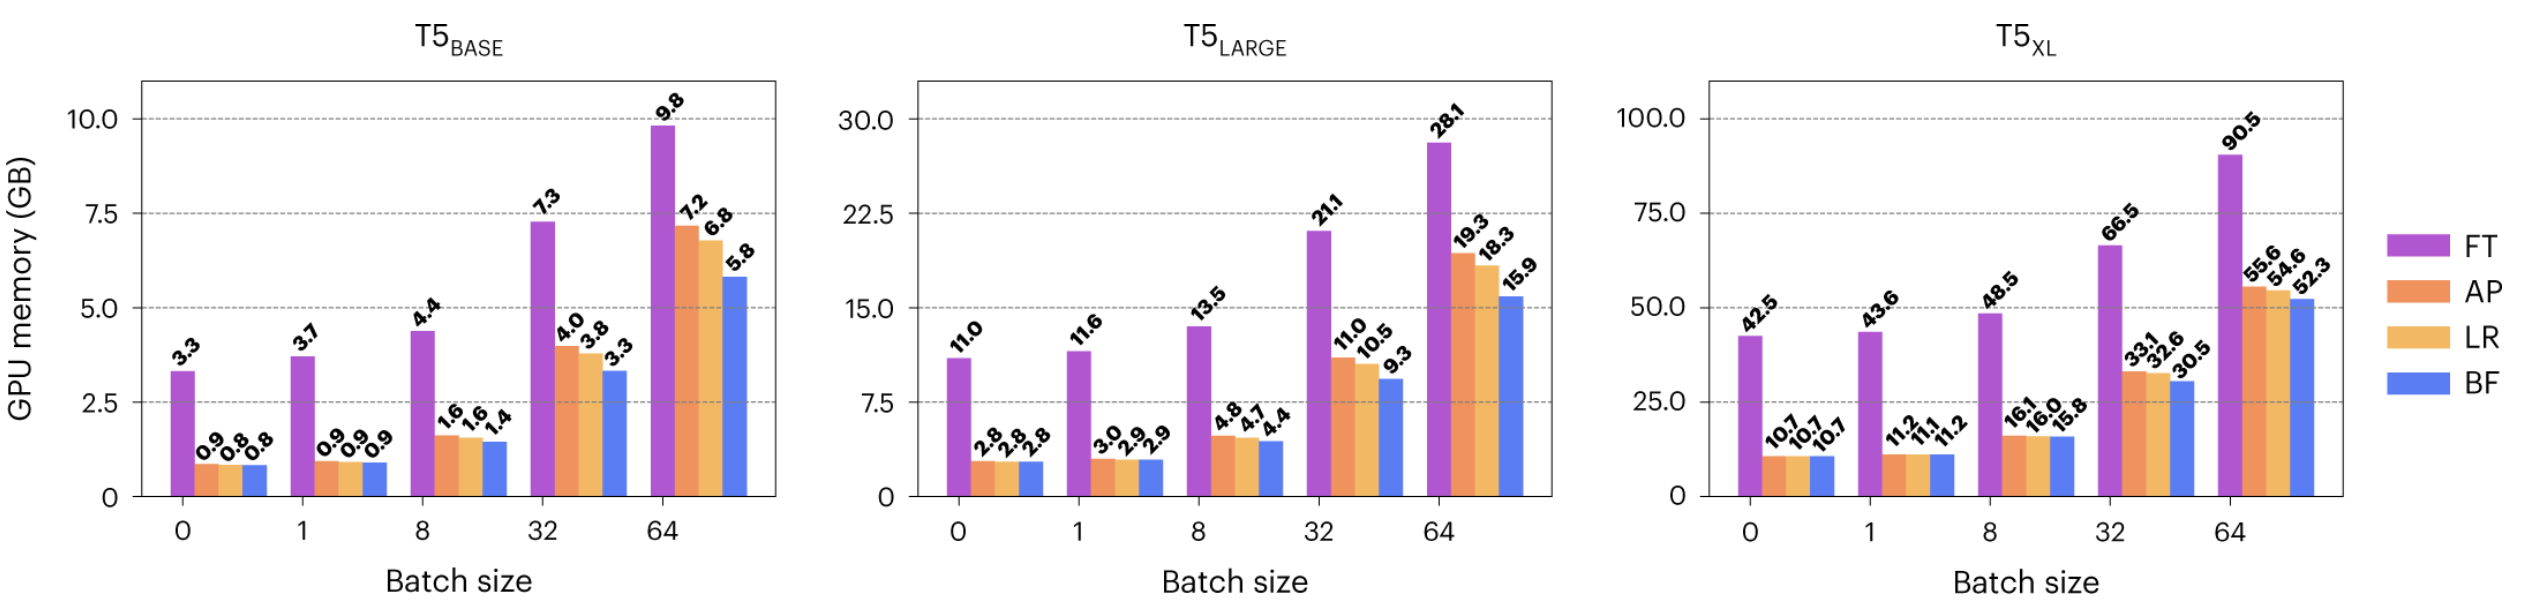
\includegraphics[width=1\textwidth]{chapter-2/peft_on_plm_memory.png}
    \caption{Perbandingan Efisiensi Memori \parencite{peft_on_plm}}
    \label{fig:peft_on_plm_memory}
\end{figure}
